The main functionality of our tool relies on runtime cost estimation procedures for several popular algorithms that can be used to solve SIS or LWE. The estimates for LWE are provided by the $\textit{estimator}$ \cite{APS15}. In addition, we included cost estimates of two different approaches for SIS. Many of the algorithms we use rely on subroutines, especially lattice reduction algorithms, and there exist more realistic and more conservative estimates. Depending on the choice of attack algorithms and reduction cost models, the returned cost may differ significantly. Also, not all attack estimates perform well in practice. It is thus of interest to us to gain a basic understanding of how the respective algorithms work.


\section{Lattice Basis Reduction}\label{sec:lattice-reduction} % perhaps move to Algorithms
% For survey see Ngu11, NV10, MW16
In \cref{sec:problems}, we showed how LWE and SIS can be viewed as lattice problems. % TODO: make sure all is there
However, the corresponding lattice basis that we obtain are rather ``ugly'' lattice bases with long basis vectors. Solving lattice problems in such a basis is infeasible. Our goal is thus to find a better basis with shorter and more orthogonal basis vectors. A family of algorithms that achieve just this is called lattice reduction algorithms.

First, we need to define a measure to evaluate the quality of a given basis. The standard measure in the literature is the (root) Hermite factor.


% % TODO: rewrite (taken from AGVW17)
% Problem: usually ugly basis (long vectors...), we want a better basis with shorter and more orthogonal basis vectors...
% - improve lattice basis quality => measure by hermite factor (compare shortest vector in basis to lattice volume) or approximation factor (compare shortest vector in basis to shortest lattice vector)
% - algorithm finding vector with approximation factor $\gamma$ can be used to solve uSVP with gap $\lambda_2(\Lambda)/\lambda_1(\Lambda) > \gamma $
% - best known theoretical bound by Slide reduction \cite{GN08a}, BKZ better in practice

% % TODO possibly put Gram-Schmidt orthogonalization here? => Size reduction algorithm and HKZ reduction, see 2.4.1 in Chen13, not sure if needed
% - measure quality of basis: Hermite factor  % TODO change or \cite{Reg10}

\begin{definition}[Root Hermite Factor \cite{LP11}]
    Given a basis $\mathbf{B} = \left\{\mathbf{b}_1, \ldots, \mathbf{b}_n\right\}$ with $\|\mathbf{b}_1\| \leq \cdots,  \leq \|\mathbf{b}_n\|$, then basis $\mathbf{B}$ has root Hermite factor $\delta$ if
    \begin{equation} \label{eq:hermite}
        \| \mathbf{b}_1 \| \approx \delta^n \det(\Lambda)^{1/n}.
    \end{equation}
\end{definition}% TODO * $\delta = 1.01$ feasible, $\delta = 1.007$ seems infeasible for now
We will later use a result that follows from the Geometric Series Assumption (GSA) as in \cite{Gop16}. The GSA estimates the length of the Gram-Schmidt vectors $\tilde{\mathbf{b}}_i$ as follows \cite{Sch03}: \label{sec:GSA} % got this from Gop16
\begin{equation} \label{eq:GSA}
    \| \tilde{\mathbf{b}}_i \| \approx \alpha^{i-1} \| \mathbf{b}_1 \|,
\end{equation}
for $0 < \alpha < 1$. If we combine \cref{eq:hermite} with \cref{eq:GSA}, we obtain  $\| \tilde{\mathbf{b}}_i \| \approx \alpha^{i-1} \delta^n \det(\Lambda)^{1/n}$. Furthermore, we know that $\prod_{i-1}^n \| \tilde{\mathbf{b}}_i \| = \det(\Lambda)$  % TODO: check
and get
\begin{align*}
    \prod_{i-1}^n \| \tilde{\mathbf{b}}_i \| \approx \prod_{i-1}^n \alpha^{i-1} \delta^n \det(\Lambda)^{1/n}
    \iff & \det(\Lambda) \approx \delta^{2n} \det(\Lambda) \prod_{i-1}^n \alpha^{i-1} \\
    \iff & \delta^{-2n} \approx \alpha^{\frac{n(n-1)}{2}}                             \\
    \iff & \delta^{-2} \approx \alpha^{(n-1)/n}
\end{align*}
Hence, $\alpha \approx \delta^{-2}$ and
\begin{equation}
    \| \tilde{\mathbf{b}}_i \| \approx \delta^{-2(i-1) + n} \det(\Lambda)^{1/n}
\end{equation}
We can see that for smaller $i$, the length of the Gram-Schmidt vectors $\tilde{\mathbf{b}}_i$ decreases, whereas for larger $i$, the length increases, resulting in a long and skinny fundamental parallelepiped $\mathcal{P}_{1/2}(\tilde{\mathbf{B}})$.


% * gap between provable and experimental cost estimate to reach some hermite $\delta$ => provable results only give upper bounds, for practical security we need lower bound => combine theoretical results with experimental results

% * well-established estimate \cite{LP11}


In the following, we will focus on two related methods for lattice reduction. % A third approach, the Hermite, Korkine, Zolotarev (HKZ) reduction %TODO: write a sentence or two about it?
First, we define some reduction criteria following \cite{ABLR21}. % TODO: sounds bad
A basis $\mathbf{B} = \left[\mathbf{b}_1 \cdots \mathbf{b}_n\right]$ is \textit{size-reduced} if its Gram-Schmidt coefficients (see \cref{sec:gram-schmidt}) satisfy $|\mu_{i,j}| \leq \frac{1}{2}$ for all $0\leq j < i < n$. If the first basis vector $\mathbf{b}_1$ of $\mathbf{B}$ is the shortest lattice vector, i.e., $\|\mathbf{b}_1\| = \lambda_1(\Lambda(\mathbf{B}))$, we call $\mathbf{B}$ \textit{SVP-reduced}. If a basis $\mathbf{B}$ is size-reduced and in addition, each block $\left\{\mathbf{b}_i, \dots, \mathbf{b}_n\right\}$ for $i=1, \dots, n$ of basis vectors is SVP-reduced, then $\mathbf{B}$ is \textit{HKZ-reduced}. We will see in the next section that size reduction is closely related to the LLL algorithm, and that a special case of the BKZ reduction outputs an HKZ-reduced basis.

% TODO: algorithm LLL reduction, check out CWX13
\subsection{The LLL Algorithm}
The LLL algorithm was proposed by Lenstra, Lenstra and Lovász \cite{LLL82} and can be considered as a generalization of the two dimensional Lagrange reduction. The Lagrange reduction reduces a basis of two basis vectors such that the output basis satisfies $\|\mathbf{b}_1\| \leq \|\mathbf{b}_2\|$ and $|\left\langle\mathbf{b}_1, \mathbf{b}_2\right\rangle| / \|\mathbf{b}_1\|^2 = |\mu_{2,1}| \leq \frac{1}{2}$. Intuitively, a multiple of the shorter vector $\mathbf{b}_1$ is subtracted from the longer vector $\mathbf{b}_2$, such that the resulting vector $\mathbf{b}_2'$ is as orthogonal to $\mathbf{b}_0$ as possible, i.e.,  $\mathbf{b}_1' =  \mathbf{b}_1 - \lfloor\mu_{1,0}\rceil \mathbf{b}_0$. We set $\mathbf{b}_2 = \mathbf{b}_2'$ and repeat until nothing changes.

A $\theta$-LLL reduced basis ensures two criteria \cite{LLL82}:
\begin{enumerate}
    \item Size-reduced: $|\mu_{i,j}| \leq \frac{1}{2}$ for $1\leq i \leq n$ and $j < i$ \label{size-red}
    \item Lovász condition: $\theta \| \tilde{\mathbf{b}}_i \|^2 > \| \mu_{i+1, i} \tilde{\mathbf{b}}_i + \tilde{\mathbf{b}}_{i+1} \|^2$ for $1\leq i < n$
\end{enumerate}

Recall the definition of the Gram-Schmidt coefficients $\mu_{i, j} = \left\langle \tilde{\mathbf{b}}_j, \mathbf{b}_i\right\rangle / \left\langle \tilde{\mathbf{b}}_j, \tilde{\mathbf{b}}_j\right\rangle$. The LLL algorithm shown in \cref{alg:LLL} follows the notation in \cite{LLLReg04}. We start by computing the Gram-Schmidt orthogonalization of the input basis (\cref{alg:LLL-start}) and continue with a reduction step in which we update every basis vector $\mathbf{b}_i$ by pairwise comparing and subtracting lower indexed basis vector, just as in the Lagrange reduction (\cref{alg:LLL-red}) to ensure Criteria \ref{size-red}. Finally, vectors violating the Lovász condition are swapped (\cref{alg:LLL-swap}) and the process is repeated until nothing changes. The LLL algorithm can be used to find short vectors of at most $2^{n/2} \lambda_1(\Lambda)$ in polynomial time. Several floating-point variants have been suggested that can significantly speed up the runtime of LLL. For example, L$^2$ runs in $\mathcal{O}(n^2 \log^2 B)$, where $B$ is a bound on the norm of the input basis vectors \cite{NS05}. % TODO: newer versions?

\begin{algorithm2e}
    \SetKwBlock{Begin}{function}{end function} % FROM https://cims.nyu.edu/~regev/teaching/lattices_fall_2004/ln/lll.pdf
    \Begin($\theta\text{-LLL} {(}\mathbf{B} \in \mathbb{Z}^{m\times n} {)}$) % TODO nxn???
    {
        Compute $\tilde{\mathbf{B}}$\label{alg:LLL-start}\\
        \For{$i=2, \dots, n$}{
            \For{$j=i-1, \dots, 1$}{
                $\mathbf{b}_i = \mathbf{b}_i - \lfloor\mu_{i, j}\rceil \mathbf{b}_j$\label{alg:LLL-red}\\
            }
        }
        \If{$\exists i \text{ \upshape such that } \theta \| \tilde{\mathbf{b}}_i \|^2 > \| \mu_{i+1, i} \tilde{\mathbf{b}}_i + \tilde{\mathbf{b}}_{i+1} \|^2$}{
            Swap $\mathbf{b}_{i}$ and $\mathbf{b}_{i+1}$\label{alg:LLL-swap}\\
            Return $\theta$-LLL($\mathbf{B}$)\\
        }
        \Else{
            Return $\mathbf{B}$\\
        }
    }
    \caption[The LLL Algorithm]{The LLL Algorithm \cite{LLL82}} \label{alg:LLL}
\end{algorithm2e}

% Theoretical and experimental output quality

The proven upper bound of the output quality of the LLL algorithm is $\delta^n = \left(4/3\right)^{\frac{n-1}{4}}$ or, equivalently, $\delta \approx 1.075$ \cite{LLL82}. In practice, we get much better results of $\delta \approx 1.021$ on average \cite{Chen13}. Given an input basis in which the length of all basis vectors is bounded by $B$, the runtime of LLL is proven to be in $\mathcal{O}\left(n^4m\log B(n+\log B)\right)$ \cite{NS05} and heuristically known to be $\mathcal{O}(n^{3}\log^2 B)$ \cite{APS15}.



\subsection{The BKZ Algorithm} \label{sec:BKZ}
% Rewrite, from Pla18

The Block Korkin-Zolotarev (BKZ) algorithm was proposed by Schnorr in 1987 and adapted by Schnorr and Euchner in \cite{SE91} and represents a family of lattice reduction algorithm. Essentially, BKZ iteratively divides the input basis into blocks of a lower dimension $k$ and calls an SVP oracle on each block. The output of the oracle is then used to obtain a basis of improved quality.

\cref{alg:BKZ} presents the main concept of BKZ and follows the description in \cite{CN11} with some adjustments. Initially, we run an LLL reduction on the input basis $\left\{\mathbf{b}_1, \dots, \mathbf{b}_{n}\right\}$ and update the basis. In each $j$th iteration, we consider a block of $k$ basis vectors $\mathbf{b}_j, \dots, \mathbf{b}_{j+k-1}$. The vectors of the current block are projected onto the orthogonal complement of $\text{span}\left(\left\{\mathbf{b}_i \mid i \in [j-1]\right\}\right)$, that is, the span of vectors from previous iterations (\cref{BKZ-span}ff; we skip this step, if the span is empty). The orthogonal complement $A^\perp$ of a subspace $A$ is defined as the set of all vectors that are orthogonal to every vector in $A$. We then run an SVP oracle on the projected block to obtain a shortest vector $\mathbf{b}_\text{new}'$ in the projected lattice (\cref{BKZ-svp}) and reconstruct a lattice vector $\mathbf{b}_\text{new}$ of which $\mathbf{b}_\text{new}'$ is a projection (\cref{BKZ-rec}). Note that in practice, the SVP oracle should include this step. If $\mathbf{b}_\text{new}$ is a new vector, we insert it in our list of basis vectors before $\mathbf{b}_j$. Otherwise, since nothing changed, we increment a counter $z$. Finally, we run LLL on all basis vectors up to index $j+i$ (including the possibly newly added vector). If no new lattice vectors can be found in $n$ iterations, the reduction terminates. After $n$ iterations, $j$ is reset to start over at the first block. The output of the algorithm is a BKZ$_k$-reduced basis. For $k=2$, we obtain an LLL-reduced basis in polynomial time, and for $k=n$, an optimally HKZ-reduced basis in at least exponential time.%TODO needed? probably not, maybe just mention k=2 case, Pla18


\begin{algorithm2e} % TODO: check if block is not of dimension kxk
    \SetKwBlock{Begin}{function}{end function}
    \Begin($\text{BKZ} {(} \mathbf{B} = \{\mathbf{b}_1, \dots, \mathbf{b}_{n}\}, k \in [n]\setminus \{1\} {)}$) % TODO nxn???
    {
            z = 0; j = 0\\
            $\mathbf{B} = \text{LLL}(\mathbf{B})$ \\% LLL reduce and update basis
            \While{$z < n-1$}{
                $j = (j \mod (n-1)) + 1; l = \min(j + k -1, n); h = \min(l + 1, n)$\\
                $A = \text{span}\left(\left\{\mathbf{b}_i \mid i \in [j-1]\right\}\right)$\label{BKZ-span}\\
                \For{$i \in \{j, ..., l\}$}{
                    \If{$A \neq \emptyset$}{
                        $\mathbf{b}_i' = \pi_{A^\perp}(\mathbf{\mathbf{b}_i})$\label{BKZ-proj}\\
                    }
                    \Else{
                        $\mathbf{b}_i' = \mathbf{b}_i$\\
                    }
                }
                $\mathbf{b}_\text{new}' = \text{SVP-Oracle}(\mathbf{b}_j', \dots, \mathbf{b}_{l}')$\label{BKZ-svp}\\
                Reconstruct $\mathbf{b}_\text{new} = \textstyle \sum_{i=j}^l\alpha_i \mathbf{b}_i$ with $\alpha_i \in \mathbb{Z}$ such that $\mathbf{b}_\text{new}' = \pi_{\left(\text{span}\left(\mathbf{b}_j, \dots, \mathbf{b}_{l}\right)\right)^\perp}(\mathbf{b}_\text{new})$\label{BKZ-rec}\\
                \If{$\mathbf{b}_\text{new}' \neq \tilde{\mathbf{b}}_j$}{
                    $z=0;$ $\{\mathbf{b}_j, \dots, \mathbf{b}_{h} \}= \text{LLL}(\{\mathbf{b}_j, \dots, \mathbf{b}_{j-1}, \mathbf{b}_\text{new}, \mathbf{b}_j, \dots, \mathbf{b}_{h} \})$\\
                }
                \Else{
                    $z = z + 1;$ $\{\mathbf{b}_j, \dots, \mathbf{b}_{h} \} = \text{LLL}(\{\mathbf{b}_j, \dots, \mathbf{b}_{h} \})$\\
                }
            }
        }
    \caption[The BKZ Algorithm]{The BKZ Algorithm \cite{SE91}} \label{alg:BKZ}
\end{algorithm2e} % TODO: check, maybe also with ABLR21, Alg 2 or 4

% TODO: explain how SVP oracle can be implemented => possibly outsource, section for cost models!!!

Several improvements have been suggested. The total number of rounds until termination is unknown and can be quite large. \citet{HPS11a} show an \textit{early termination} of BKZ still yields a very good output basis quality and propose $\frac{n^2}{k^2} \log n$ rounds as a bound.

\textit{Local preprocessing} increases the quality of the current block basis by recursively calling BKZ with smaller block size. A variant known as \textit{progressive BKZ} applies the recursion globally \cite{AWHT16}.

If enumeration is used as an SVP oracle, the size of the search space can be reduced by means of \textit{pruning} techniques. Nodes closer to the edges of the enumeration tree are less likely to result in short lattice vectors. For more details on enumeration, we refer to \cref{sec:enumeration}. \citet{GNR10} show that applying a variant of this known as \textit{extreme pruning} can reduce the running time by a much larger factor than the success probability. Repeating the search yields the desired speedup.

In addition, \cite{CN11} optimizes the \textit{enumeration radius} by using experimental results. BKZ 2.0 incorporates a number of these techniques \cite{CN11}.

% BKZ runtime bounds: TODO rewrite, from MW16
% - runtime (without early termination) grows superpolynomially in $n$ \cite{GN08b}
% - best provable bounds on ouput after termination worse than that of slide reduction by at least polynomial factor (slide reduction [\cite{GN08a}] yields best theoretical results but in practice worse than BKZ)
% - calls to SVP oracle in arbitrary dimensions up to block size => runtime depends on worst-case Hermite constants of each block size 
% => simulation of BKZ needs to include estimation of runtime of SVP oracle for each block size
% TODO: use the following? 
% Versions:
% - slide reduction yields best theoretical result (2^n log log n /log n) \cite{GN08a} 
% - practical floating point version of LLL \cite{SE91} best practical results 

It is difficult to find hard runtime bounds for BKZ. The upper bound on the number of rounds is superexponential in the dimension $n$ for a fixed block size \cite{HPS11a, GN08b} before BKZ terminates, given that no early termination strategy is used. In addition, calls to the SVP oracle in all dimensions $k' \leq k$ must be considered.
\citet{APS15} ignore these intricacies and estimate the cost of BKZ in clock cycles as $\rho \cdot n \cdot t_k$, where $\rho$ is the number of rounds needed and $t_k$ is the cost (in block cycles) of calling the SVP oracle on a block of dimension $k$. The value $\rho$ is set to $8$ in the \textit{estimator} and is derived from experiments in \cite{Chen13} that indicate that the most significant progress happens in the first $7-9$ rounds. \label{sec:bkz-8d}

% TODO: output quality: 
The output quality of BKZ is closely related to the used block size $k$. The \textit{estimator} uses a limiting value from \cite{Chen13} to estimate the root Hermite factor $\delta$ for a given $k$:
\begin{equation}
    \lim_{n\rightarrow \infty} \delta \approx \left( \frac{k (\pi k)^{\frac{1}{k}}}{2\pi e}\right)^{\frac{1}{2(k-1)}}
\end{equation}
For smaller block sizes $k\leq 40$, the \textit{estimator} uses fixed experimental values for $\delta$.
% TODO: include? \cite{LP11} runtime according Linder-Peikert model, GSA: suggest $t_{\text{BKZ}}=1.8/\log_2{\delta} - 110$


% TODO perhaps look into: General Sieve Kernel implementation \cite{ADHKPS19} beats BKZ + pruned enum 



\subsection{Cost Models for Lattice Reduction} \label{sec:costmodels}
% TODO. write little introduction
In this section, we will look at various high-level ideas to realize an SVP solver that can be used as a subroutine in BKZ and present up-to-date cost models from the literature. SVP is known to be NP-complete even for large constant approximation factors \cite{Ajt98, Khot05}. An exponential approximation factor can be achieved in polynomial time, but is mostly insufficient for practical purposes \cite{LLL82}.  We will mainly focus on two classes of (nearly) exact SVP solvers, namely, enumeration algorithms and sieving algorithms. Enumeration algorithms can solve SVP in a lattice of dimension $k$ in $2^{\mathcal{O}(k \log k)}$ time and polynomial space. Sieving algorithms only need $2^{\mathcal{O}(k)}$ time, however, at the cost of exponential memory complexity. Only recently, progress in sieving strategies has given rise to BKZ implementations relying on sieving (e.g., the General Sieve Kernel (G6K) implementation \cite{ADHKPS19, DSW21}) that outperform enumeration implementations already in relatively small dimensions $\gtrsim 70$ in the classical setting \cite{ABLR21}. On the other hand, quantum speedups for enumeration are greater than for sieving. \citet{ANS18} show a quadratic cost reduction for enumeration, while the speedup is much lower for sieving, even with idealized assumptions \cite{Laa15}. The authors of \cite{ADPS16} argue that due to a lower bound $2^{0.2075k}$ on the required size of the building lists, future quantum sieving algorithms are not expected to achieve an asymptotic runtime below $2^{0.2075k}$. % assuming no depth restriction and quantum accessible RAM (qRAM)

A selection of the most relevant cost models for cryptographic purposes can be seen in \cref{tab:costmodels}. All of these cost models are supported in our tool (see \cref{sec:tool-costmodels}).


% nice overview in https://cseweb.ucsd.edu/~daniele/LatticeLinks/Enum.html
\subsubsection{Enumeration} \label{sec:enumeration}% see Chen13 for a better explanation
Enumeration aims to find the shortest vector by enumerating all lattice vectors within some bounded region. In general, we start with reducing the lattice basis to improve the basis quality. We then define a bound and iteratively project the lattice to the span of its Gram-Schmidt vectors beginning from $\tilde{\mathbf{b}}_n$ until we arrive at the lowest level of a one-dimensional subspace. We continue by enumerating all vectors of norm less than $r$ in the projected lattice and ``lift'' each of these vectors to the level above and repeat this process until we arrive at the level from which we started. The search space can be thought of as a large tree of (projected) vectors on which we apply depth-first search. Note that the root of the tree here is at the lowest level and the leaves are the lattice vectors in our target lattice. %Consider a two-dimensional lattice with basis $\left\{\mathbf{b}_1, \mathbf{b}_2 \right\}$ and bound $r = \| \mathbf{b}_1 \|$. We project the lattice to the span of the Gram-Schmidt vector $\tilde{\mathbf{b}}_2$ and enumerate all the vectors within the  $r$... Not really needed
The low memory cost of enumeration is due to its similarities to depth-first search.

A very early but very efficient variant was suggested by \citet{Kan83} with a proven worst-case runtime of $2^{\mathcal{O}(k \log k)}$. BKZ$_k$ using Kannan's enumeration algorithm as SVP oracle yields a short lattice vector of norm approximately $\left(k^{1/(2k)}\right)^n\cdot \text{det}(\Lambda)^{1/n}$, or equivalently achieves a root Hermite factor of $k^{1/(2k)}$ \cite{HS07, ABFKSW20}. % TODO check if n or m
% TODO: write sth about root hermite factor, ... for the next sections or change next sections

In \cite{ABFKSW20}, we find a more concrete experimental cost model of $\text{poly}(n) \cdot 2^{(k \log k) / (2e)  - 0.995 k + 16.25}$ for BKZ 2.0 (see \cref{sec:BKZ}), where $\text{poly}(n)$ is the number of calls to the enumeration subroutine. BKZ 2.0 achieves a  root Hermite factor of $\left(k / (2\pi e) \cdot (\pi k)^{1/k}\right)^{1 / (2(k-1))}$ \cite{Chen13}.

% TODO add to BKZ variants!!! => extended preprocessing and relaxing of search radius, 
% also add G6K (General Sieve Kernel) from ADHKPS19 (see more in sieving), running time of 2^Theta(k) but also 2^Theta(k) memory
The FastEnum algorithm in \citet{ABFKSW20} incorporates an idea called ``extended preprocessing'' and simulations achieve a root Hermite factor of $k^{(1 + o(1))/(2k)}$ in $\text{poly}(n) \cdot 2^{0.125k \log k - 0.050k + 56}$ time. The corresponding quantum algorithm reduces the runtime from $2^{(k \log k)/8 + o(k)}$ to $2^{(k \log k) / 16 + o(k)}$. In extended preprocessing, instead of preprocessing the current projected basis block of size $k$, the BKZ-reduction is applied to a block of higher dimension $\lceil (1+c)\cdot k\rceil$ for some constant $c$. Enumeration is faster on the first basis vectors, as their Gram-Schmidt norms closely follow the Geometric Series Assumption \cite{MW16}. % TODO: move to BKZ ??? And perhaps switch BKZ with this section?

A tradeoff of runtime and success probability for ``relaxing'' the approximation and extreme pruning turns out to exponentially speed up the search \cite{LN20} and was combined with extended preprocessing by \citet{ABFKSW20} to further reduce the experimental runtime of BKZ to $\text{poly}(n) \cdot 2^{(k \log k)/8 - 0.654k + 25.84}$ for a root Hermite factor of $k^{1/(2k)}$.

% TODO: what to do with poly(n)? just throw it away? 


% TODO: for table
% BKZ 2.0 & \cite{CN11, Chen13, ABFKSW20} & $2^{0.184k \log k - 0.995k + 16.25}$
% ABF+ Enum & \cite{ABFKSW20} & $2^{0.125k \log k}$ => root Hermite factor of $k^(1/(2k))$
% ABF+ Enum + O(1)& \cite{ABFKSW20} & $2^{0.125k \log k - 0.547k + 10.4}$
% ABF Q-Enum & \cite{ABFKSW20} & $2^{0.0625 k \log k}$ 
% ABLR Enum + O(1)& \cite{ABLR21} & $2^{0.125k \log k - 0.654k + 25.84}$



\subsubsection{Sieving}
The second group of SVP solvers are sieving algorithms \cite{ADHKPS19, MV10, NV08, BGJ15, BLS16, HK17,BDGL16}. In sieving, initially, we create a long list of randomly selected lattice points. The points in the list are then combined or ``reduced'' in some way to find points of smaller length. One way to achieve this is by finding a minimal sublist of ``center'' points in the initial list, such that spheres centered at these points cover all list points. Subtracting the center points yields short lattice points. ListSieve \cite{MV10} uses a smaller initial list to divide the space into two half-spaces, one closer to the center and one closer to the respective point. The list is then used to reduce the length of newly sampled points as much as possible by subtracting each list vector, such that the result is located in the half-space closer to the center. Once two points with a distance less than the target distance are found, they are subtracted, and the result is returned.
% TODO: nearest neighbor speedups: combining two vectors can only result in reduction only if their pairwise angle is less than $60°$. A candidate check of two vectors of similar length can thus be carried out by testing if the angle is at most $\pi/3$. \cite{BDGL16}

% nice overview and explanation in \cite{ADHKPS19}
\begin{table}[h]
    \centering
    \begin{tabular}{lll}
        \toprule
        Algorithm                                & Runtime complexity   & Memory complexity    \\\hline
        List Sieve \cite{MV10}                   & $2^{0.3199n + o(n)}$ & $2^{0.1325 + o(n)}$  \\
        NV-sieve \cite{NV08, ADHKPS19}           & $2^{0.415n + o(n)}$  & $2^{0.2075n + o(n)}$ \\
        NV-sieve (quantum) \cite{NV08, ADHKPS19} & $2^{0.311n + o(n)}$  & $2^{0.2075n + o(n)}$ \\
        Gauss sieve \cite{MV10, HK17}            & $2^{0.415n + o(n)}$  & $2^{0.2075n + o(n)}$ \\
        BGJ-sieve \cite{BGJ15}                   & $2^{0.311n + o(n)}$  & $2^{0.2075n + o(n)}$ \\
        3-sieve \cite{BLS16, HK17}               & $2^{0.3962n + o(n)}$ & $2^{0.1887n + o(n)}$ \\
        BDGL-sieve \cite{BDGL16}                 & $2^{0.292n + o(n)}$  & $2^{0.2075n + o(n)}$ \\
        BDGL-sieve (quantum) \cite{BDGL16}       & $2^{0.265n + o(n)}$  & $2^{0.2075n + o(n)}$ \\
        \bottomrule
    \end{tabular}
    \caption{Overview of Popular Sieving Algorithms} % TODO: cite? from estimate all the?
    \label{tab:sieving}
\end{table}

\cref{tab:sieving} presents a list of currently best sieving algorithms. Note that some runtime and space complexities are only conjectured and not proven yet.

In the Nguyen-Vidick sieve \cite{NV08}, we iteratively reduce a pair of list points whose combined length is smaller than the longest list vector. The longest vector is then replaced by the result. The list length is fixed.
In the Gauss sieve \cite{MV10}, we start with an empty list and a stack. In each step, a new point is either sampled or taken from the stack. We then attempt to reduce the new point with all points in the list. If a reduction is successful, the longer vector of the pair is replaced. If the longer vector was the list point, the replacement is inserted in the stack. If no reduction is possible, the stack points are moved back to the list. If the stack is empty, all list points are reduced pairwise. In practice, the Gauss sieve outperforms Nguyen-Vidick sieve.
The Becker-Gama-Joux sieve \cite{BGJ15} exploits coding theory to find vectors that are likely to be nearest neighbors. Similar vectors are stored in the same bucket to speed up the search for reduction candidates.
The 3-sieve \cite{BLS16, HK17} reduces the required list size by using triples instead of pairs of points for combination.
Finally, the Becker-Ducas-Gama-Laarhoven sieve \cite{BDGL16} applies locality sensitive hashing to create buckets of points in near neighborhood similar to the Becker-Gama-Joux sieve. % CHECK if that is ListDecoding








% TODO: check out AKS01 algorithm 

% recent progress: % from DSW21
% - theoretical: Laa15, BGJ15, BDGL16, HKL1
%   techniques: 
%     Nearest Neighbor Search (Laa15)
%     Progressive Sieving (LM18)
%     Dimensions for Free (Duc18): lift many short vectors in sieving dimension to recover short vector in larger dimensions
% - practical performance: FBB+14, Duc18, LM18, ADHKPS19

% quantum: sieving uses near neighbor search as subroutine, which in turn uses black box search, Grover's quantum search algorithm reduces the complexity of black box search by square root \cite{Gro97}


% TODO also check out LM18, Duc18, ADHKPS19



%of length smaller than some bound $r$. Then, we choose some center points $\mathbf{v}'_i, i \in [l]$ for some $l \ll 2^{cn}$ of the list such that all points $\mathbf{v}_i$ of the initial list are covered by spheres of a radius $r' < r$ centered at these center points $\mathbf{v}'_i$. Finally, we compute short vectors by subtracting the centers. % TODO


% - CN11, APS15, ADPS16
% sieving \cite{BDGL16, Laa15,ADPS16, APS15,BDGL16}
% enumeration \cite{Kan87, MW15,FP85, CN11, APS15, HPSSWZ17}
% cost models (tabular overview) \cite{ACCD+19}
% - number of SVP calls \cite{ADPS16,Alb17}
% - upper bound on rounds is exponential \cite{HPS11a, GN08b}
% - lattice rule of thumbs: achievable root hermite factor $\delta_0 = k^{\frac{1}{2k}} $ % [Stehlé12 An introduction to lattice reduction] or 2^1/k [Stehlé13/16  An overview of lattice reduction algorithms] (oversimplification)





% primarily studied for SVP in euclidean norm
% two main types: 
% Classic Sieve \cite{AKS01}: create a long list of lattice vectors, then find shorter lattice vectors and discard longer
% List Sieve \cite{MV10}: start from empty list, find shorter vectors and append them to list

% best provable: $2^{n + o(n)}$ (sieving by averages)
% heuristic state of the art: $(3/2)^{n/2 + o(n)} \approx 2^{0.29n}$ 

% combinarial: create list of short random (possibly non-lattice) vectors, try to combine vectors in list to produce short lattice vectors
% provable versions not very useful (exponential space, random perturbations) but basis of heuristic variants used in practice 


% TODO: decide whether to take others
% \subsubsection{Others}
% - discrete Gaussian sampling % \cite{ADRS15}, adps?
% % TODO insert a table and reference somewhere else? Warum notwendig, wie kommt man darauf? ... alg laufen lassen, extrapolieren...
% - Micciancio-Voulgaris Algorithm - Voronoi-cell algorithm \cite{MV13} in $4^{n + o(n)}$ time and $2^{n+o(n)}$ space


% TODO: make chronology? 
% \begin{figure}
%   \begin{chronology}[5]{2000}{2021}{3ex}[\textwidth]
%     \event{2001}{AKS sieve $2^{\mathcal{O(n)}}$ time and space \cite{AKS01}}
%     \event{2010}{List sieve in $2^{3.2n}$ time and $2^{1.33n}$ space \cite{MV10}}
%     \event{2013}{Voronoi cell $2^{2n}$ time and $2^{n}$ space \cite{MV13}}
%     \event{2014}{Gaussian sampling $2^{n}$ time and space \cite{ADRS14}}
%   \end{chronology}
%   \caption{Provable algorithms for SVP}
% \end{figure}

\begin{table}
    \centering
    \begin{tabular}{lll}
        \toprule
        Name                             & Reference                       & Cost model                            \\\hline
        Sieving                          &                                 &                                       \\\hline
        Q-Sieve (paranoid lower bound)   & \cite{ADPS16}                   & $2^{0.2075k}$                         \\
        Q-Sieve                          & \cite{Laa15,ADPS16,AGPS20}      & $2^{0.265k}$                          \\
        Q-Sieve + O(1)                   & \cite{SAL+17}                   & $2^{0.265k + 16}$                     \\
        Q-Sieve (min space)              & \cite{SHRS17}                   & $2^{0.2975k}$                         \\
        Sieve                            & \cite{BDGL16,ADPS16,AGPS20}     & $2^{0.292k}$                          \\
        Sieve + O(1)                     & \cite{SAL+17}                   & $2^{0.292k + 16}$                     \\
        Sieve (min space)                & \cite{SHRS17}                   & $2^{0.368k}$                          \\\hline
        Enumeration                      &                                 &                                       \\\hline
        Lotus                            & \cite{PHAM17, ACDDPPVW18}       & $2^{0.125k \log k - 0.755 k + 2.254}$ \\
        Enum + O(1)                      & \cite{SHRS17,Chen13,ACDDPPVW18} & $2^{0.187k \log k - 1.019 k + 16.1}$  \\
        Q-Enum + O(1)                    & \cite{SHRS17,Chen13,ACDDPPVW18} & $2^{0.0936k \log k - 0.51 k + 8.05}$  \\
        BCLV-Enum (quadratic fit) + O(1) & \cite{BCLV17}                   & $2^{0.000784 k^2 + 0.366 k + 0.875}$  \\
        BKZ2.0-Enum                      & \cite{CN11, Chen13, ABFKSW20}   & $2^{0.184k \log k - 0.995k + 16.25}$  \\
        ABF-Enum                         & \cite{ABFKSW20}                 & $2^{0.125k \log k}$                   \\
        ABF-Enum + O(1)                  & \cite{ABFKSW20}                 & $2^{0.125k \log k - 0.547k + 10.4}$   \\
        Q-ABF-Enum                       & \cite{ABFKSW20}                 & $2^{0.0625 k \log k}$                 \\
        ABLR-Enum + O(1)                 & \cite{ABLR21}                   & $2^{0.125k \log k - 0.654k + 25.84}$  \\
        \bottomrule
    \end{tabular}
    \caption[SVP Cost Models Overview]{SVP Cost Models Overview (Based on \cite[Table~4]{ACDDPPVW18})} % TODO: cite? from estimate all the?
    \label{tab:costmodels}
\end{table} % TODO: add to tool, maybe change 8d thing to an optional parameter!!! => reduces number of lists, throw out silly ones...
% TODO reference in text
% TODO: add description of "core"










\section{Algorithms for Solving LWE}
In this section, we present a number of popular attacks on LWE. The \textit{estimator} includes cost estimate algorithms for each of these attacks. In our treatise, we will ignore special cases of LWE that can be exploited to obtain more efficient attack variants and only present the main algorithms. For more details, we refer the reader to \cite{APS15} and \cite{BBGS19}.

\subsection{Lattice Problems}
Some of the following attacks rely on a reduction of LWE to different lattice problems. We first define three important lattice problems in the context of LWE.

\begin{definition}[HSVP$_\delta$] \label{def:hsvp}
    Given a basis $\mathbf{B}$ of a lattice $\Lambda(\mathbf{B}) \in \mathbb{R}^m$, the (approximate)  Hermite Shortest Vector Problem (HSVP$_\delta$) is the problem of finding a nonzero lattice vector $\mathbf{v} \in \Lambda$ such that $\| \mathbf{v} \| \leq \delta \cdot \text{det}(\Lambda)^{\frac{1}{n}}$.
\end{definition}

\begin{definition}[uSVP$_\gamma$] \label{def:usvp}
    Given a lattice $\Lambda$ such that $\lambda_2(\Lambda) > \gamma \lambda_1(\Lambda)$, the (approximate) Unique Shortest Vector Problem (uSVP$_\gamma$) is the problem of finding the shortest nonzero vector in $\mathbf{v} \in \Lambda$ with $\|\mathbf{v}\| = \lambda_1(\Lambda)$.
\end{definition}
% or more relaxed version $\|\mathbf{v}\| = \gamma\lambda_1(\Lambda)$
%NP hard when $\gamma = 1 + 2^{-n^c}$ for some constant $c$ \cite{KS01}

\begin{definition}[BDD$_\gamma$] \label{def:bdd}
    Given a lattice $\Lambda \subset \mathbb{R}^m$ and a target vector $\mathbf{t}\in\mathbb{R}^m$ such that $\text{dist}(\mathbf{t}, \Lambda) < \gamma \lambda_1(\Lambda)$, the (approximate)  Bounded Distance Decoding (BDD$_\gamma$) is the problem of finding the closest lattice vector $\mathbf{v} \in \Lambda$, i.e., $\mathbf{v} = \argmin_{\mathbf{v}' \in \Lambda} \|\mathbf{v}' - \mathbf{t}\|$.
\end{definition}

% or more relaxed version: find closest vector $\mathbf{v} \in \Lambda$ such that $\|\mathbf{v} - \mathbf{t}\| < \gamma \lambda_1(\Lambda)$
% alternate NP hard for $\gamma > 1/\sqrt{2}$ \cite{LLM06}


\subsection{Approaches}
\cref{fig:algorithms} gives an overview of the three main approaches to solving LWE. The most natural approach is to recover the secret in LWE directly, e.g., by exhaustively searching the search space. In general, however, the search space is quite large, resulting in high attack costs. The \textit{estimator} incorporates two direct attacks, the Meet-in-the-Middle attack \cite{BG14} and an attack due to Arora and Ge \cite{AG11}. % TODO Arora Ge is not exhaustive search.... 
% Overview in BBGS19
\begin{figure}[h]
    \centering
    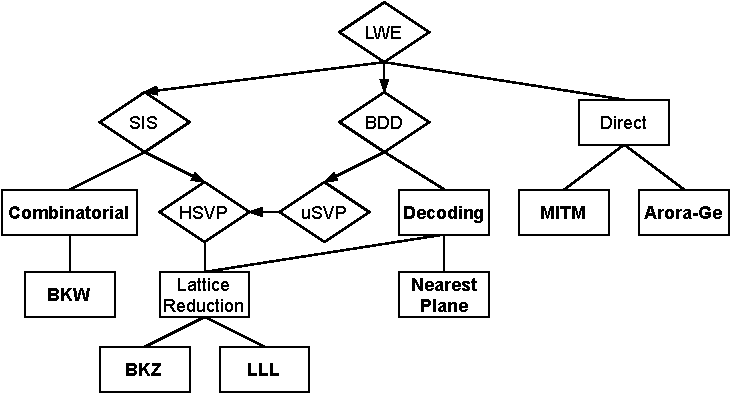
\includegraphics[width=0.9\textwidth]{graphics/algorithms_overview.pdf}
    \caption[An Overview of Algorithms and Related Problems for Solving LWE]{An overview of algorithms and related problems for soling LWE in this work. The diamond shaped boxes represent problems and arrows reductions between problems. Rectangular boxes represent approaches, classes of algorithms or algorithms. A connection between a problem and a rectangular box indicates that the latter can be used as a solver for the respective problem. Bold names indicate algorithms that can be used in our tool.}\label{fig:algorithms}
\end{figure}

\subsubsection{Primal Attack}\label{sec:primal-attacks}
The second approach aims to solve LWE in the primal LWE lattice by a reduction to the BDD problem. Consider an LWE instance with samples $\mathbf{A}, \mathbf{z}$ and the corresponding lattice $\Lambda_q(\mathbf{A}^\intercal)$. We know that for the secret vector $\mathbf{s}$ and error vector $\mathbf{e}$, it holds that $\mathbf{z} = \mathbf{A}^\intercal \mathbf{s} + \mathbf{e} \mod q = \mathbf{A}^\intercal \mathbf{s} + \mathbf{e} + q \mathbf{x}$ for some vector $\mathbf{x} \in \mathbb{Z}^m$. Obviously, $\mathbf{A}^\intercal \mathbf{s} + q \mathbf{x}$ is a lattice vector in the lattice $\Lambda_q(\mathbf{A}^\intercal)$. We know that $\text{dist}(\mathbf{z}, \Lambda_q(\mathbf{A}^\intercal) = \|\mathbf{e}\|$ and in general, it holds that $\|\mathbf{e}\| < \gamma \lambda_1(\Lambda_q(\mathbf{A}^\intercal))$. We thus have a reduction from LWE to BDD. By finding closest lattice point to $\mathbf{z}$ or, in other words, solving BDD in the lattice $\Lambda_q(\mathbf{A}^\intercal)$ we obtain $\mathbf{A}^\intercal \mathbf{s} + q \mathbf{x}$  and can recover the secret $\mathbf{s}$.

\subsubsection{Dual Attack}\label{sec:dual-attacks}
Finally, we can take advantage of the close relationship of LWE and SIS and solve LWE by finding a short vector in the dual SIS lattice \cite{LP11}. More precisely, we want to find a short nonzero vector $\mathbf{v}\in \mathbb{Z}_q^{m}$ in the scaled $q$-ary lattice $\Lambda_q(\mathbf{A}^\intercal)^{\perp} = \{ \mathbf{y} \in \mathbb{Z}^m \mid \mathbf{A} \mathbf{y} = \mathbf{0} \mod q\}$. Obviously, we have that $\langle \mathbf{v}, \mathbf{z} \rangle = \langle \mathbf{v}, \mathbf{A}^\intercal \mathbf{s} \rangle + \langle \mathbf{v}, \mathbf{e}\rangle = \langle \mathbf{v}\mathbf{A}^\intercal,  \mathbf{s} \rangle + \langle \mathbf{v}, \mathbf{e} \rangle = \langle \mathbf{v}, \mathbf{e} \rangle \mod q $ and $\langle \mathbf{v}, \mathbf{z} \rangle$ roughly corresponds to a sample drawn from a Gaussian with parameter $s' = \|\mathbf{v}\| \cdot s$, given that $\mathbf{e}$ is distributed according to a Gaussian with parameter $s$. We then test whether $\langle \mathbf{v}, \mathbf{z} \rangle \mod q$ approximates the Gaussian. If $\mathbf{z}$ is instead drawn from a uniform distribution, the test accepts exactly with probability $0.5$ \cite{LP11}. If $s'$ is not much larger than $q$, the advantage of distinguishing uniform from LWE samples is very close to $\exp(-\pi (\| \mathbf{v} \| s/q)^2)$. An optimal attack cost can be achieved by balancing the advantage with the computational effort required to solve SVP$_\gamma$ on the SIS lattice, where $\gamma = \|\mathbf{v}\|$.
% TODO from LP11, change
% TODO: maybe include graphic of three approaches

% Distinguishing attacks (MR09, RS10): distinguish (with noticeable advantage) LWE instance from uniformly random (Decision-LWE) => break semantic security of LWE-based cryptosystem with same advantage (typically)

% advantage an computational effort need to be balanced (often inverse distinguishing advantage is in total cost of attack)




% \subsubsection{Direct} % or combinatorial

% % TODO: based on GSJ15, rephrase
% - algebraic approach Arora and Ge with subexponential complexity when $\sigma \leq \sqrt{n}$, else fully exponential, mainly of asymptotic interest (higher complexity than others)
% - Exhaustive Search





\subsection[Decoding Attack]{Decoding Attack \cite{LP11}} \label{sec:decoding}
% TODO category?

The decoding attack falls into the regime of primal attacks that solve LWE by solving BDD in the primal LWE lattice (as described in \cref{sec:primal-attacks}). In the decoding attack, we first apply a reduction algorithm to the input basis $\mathbf{A}^\intercal$ to improve the basis quality. We then enumerate a number of candidate lattice points close to our target $\mathbf{z}$ by running a variant of Babai's Nearest Planes algorithm and simply choose the closest point. % TODO
% TODO: bounded distance decoding, explain more?

% (bounded-distance decoding with preprocessing?) => time/success tradeoff
% specifically for LWE, exploits structural properties of LWE


% on search version of LWE problem, approach preferable to distinguishing attack on decision LWE in \cite{MR09, RS10}, same or better advantage than distinguishing attack using lattice vectors of lower quality => runtime is smaller % This is not true anymore. Primal uSVP has become comparable (\cite{Gop15}) 
% post-reduction: simple extension of Babai's ``nearest-Planes'' algorithm \cite{Bab85} % TODO describe
% => trade basis quality against decoding time
% related to Klein's (de)randomized algorithm \cite{Kle00} for bounded-distance decoding

% use entire reduced basis, post-reduction part is fully parallelizable
% prerequisites: babai's nearest Planes algorithm (at least describe textually?), fundamental parallelepiped P_1/2



We begin with the original Nearest Planes algorithm due to Babai \cite{Bab85}, as shown in \cref{alg:babai}. Our algorithm follows the notation in \cite{NPReg04}. The goal of the algorithm is to find a lattice vector relatively close to the target vector. The procedure used is similar to the procedure in the inner loop of LLL. We first project $\mathbf{t}$ to the span of all basis vectors $\text{span}(\mathbf{B})$, where $B$ denotes an LLL-reduced basis, to eliminate irrelevant dimensions and obtain a projected vector which we call $\mathbf{b}$. Next, we iterate over $i=n, \ldots, 1$. In each step, we want to find the closest hyperplane $c_i \tilde{\mathbf{b}}_i + \text{span}(\mathbf{b}_1, \dots, \mathbf{b}_{i-1})$ to the projected vector $\mathbf{b}$. We can compute $c_i$ by a simple projection of $b$ onto the Gram-Schmidt vector $\tilde{\mathbf{b}}_i$ and dividing by the square length of $\tilde{\mathbf{b}}_i$. We subtract $c_i \mathbf{b}_i$ from $b$ and replace $\mathbf{b}$ with the result. Notice that in the last step, the hyperplane is simply a point. We return $\mathbf{t} - \mathbf{b}$. If we indeed found the closest lattice vector for target $\mathbf{z}$, the vector $\mathbf{b}$ will be our error vector $\mathbf{e}$ and $\mathbf{t} - \mathbf{b}$ will be the desired lattice vector  $\mathbf{A}^\intercal \mathbf{s} + q \mathbf{x}$, from which we can recover our secret.

\begin{algorithm2e}
    \SetKwBlock{Begin}{function}{end function}
    \Begin($\text{NearestPlanes} {(}\text{LLL-reduced basis }\mathbf{B} \in \mathbb{R}^{m \times n},\text{ target }\mathbf{t}\in \mathbb{R}^{m}{)}$)
    {
        $\mathbf{b} = \pi_{\text{span}(\mathbf{B})}(\mathbf{t})$\\
        \For{$i = n, \dots, 1$}{
            $c_i = \text{round}(\langle \mathbf{b}, \tilde{\mathbf{b}}_i\rangle /  \langle \tilde{\mathbf{b}}_i, \tilde{\mathbf{b}}_i\rangle)$\\
            $\mathbf{b} = \mathbf{b} - c_i \mathbf{b}_i$\\
        }
        output $\mathbf{t} - \mathbf{b}$\\
    }
    \caption[Babai's Nearest Planes Algorithm]{Babai's Nearest Planes Algorithm \cite{Bab85}}\label{alg:babai} % TODO change algorithm to match below or just take intuitive description
\end{algorithm2e}

In general, however, the output is a lattice vector $\mathbf{v} \in \Lambda(\mathbf{B})$ in the fundamental parallelepiped of the Gram-Schmidt basis $\mathcal{P}_{1/2}(\tilde{\mathbf{B}})$ and we only get the guarantee of $\|\mathbf{v} - \mathbf{t}\| \leq 2^{n/2} \text{dist}(\mathbf{t}, \Lambda(\mathbf{B}))$. To apply the algorithm on LWE, either $\mathbf{e}$ must be in $\mathcal{P}_{1/2}(\tilde{\mathbf{B}})$ or we must increase our search radius. The former case is unlikely as the last Gram-Schmidt vectors in a reduced basis because of the long and skinny structure of $\mathcal{P}_{1/2}(\tilde{\mathbf{B}})$ (see \cref{sec:GSA}). The latter case is exactly what the generalized algorithm by \cite{LP11} does.

Instead of choosing only the nearest plane in each iteration step, the Lindner and Peikert's variant that can be seen in \cref{alg:GeneralizedNearestPlanes} selects a variable amount $d_k$ of distinct planes in each step. As a consequence, the fundamental parallelepiped of the Gram-Schmidt basis is stretched in the direction of $\tilde{\mathbf{b}}_k$. The values of $\mathbf{d}$ should be chosen such that the covered area is approximately the same in each direction (i.e., by maximizing $\min_i(d_i \cdot \|\tilde{\mathbf{b}}_i\|)$). In particular, this implies that the $d_k$ are larger for larger $k$, as the Gram-Schmidt vectors have a smaller length. % TODO combine with section above 
Compared to \cref{alg:babai}, the runtime increases by a factor $\prod_{i \in \{1, \dots, d_k\}} d_i$; however, the recursion step can be fully parallelized.

\begin{algorithm2e}
    \SetKwBlock{Begin}{function}{end function}
    \Begin($\text{GeneralizedNearestPlanes} {(} \mathbf{B} \in \mathbb{R}^{m \times k},\mathbf{t} \in \mathbb{R}^{m}, \mathbf{d} \in {(}\mathbb{Z}^+{)}^k {)}$)
        { % TODO make sure that basis is always R^n, not Z^n
        \If{k = 0}{
            Return $\mathbf{0}$\\
        }
        \Else{
        Compute projection $\mathbf{v}$ of $\mathbf{t}$ onto $\text{span}(\mathbf{B})$\\
        Compute the $d_k$ distinct integers $c_1, \dots, c_{d_k}$ closest to $\langle \mathbf{v}, \tilde{\mathbf{b}}_k\rangle /  \langle \tilde{\mathbf{b}}_k, \tilde{\mathbf{b}}_k\rangle$\\
        Return $\bigcup_{i \in \{1, \dots, d_k\}} (c_i \cdot \mathbf{b}_k + \text{GeneralizedNearestPlanes}(\{\mathbf{b}_1, \dots, \mathbf{b}_{k-1}\}, (d_1, \dots, d_{k-1}), \mathbf{v} - c_i \cdot \mathbf{b}_k))$\\
    }
    }
    \caption[Generalized Nearest Planes Algorithm]{Generalized Nearest Planes Algorithm \cite{LP11}}\label{alg:GeneralizedNearestPlanes}
\end{algorithm2e}

It is evident that a lower quality of the reduced input basis can be compensated by increasing the values of $\mathbf{d}$. The input parameters of the lattice reduction and the generalized Nearest Planes algorithm should hence be adjusted such that the overall runtime is minimized. % TODO perhaps reformulate
% TODO: add exact success probability? 
The success probability of the Generalized Nearest Planes algorithm is given by
\begin{equation*}
    \text{Pr}\left[ \mathbf{e} \in \mathcal{P}_{\frac{1}{2}}(\tilde{\mathbf{B}} \cdot \text{diag}(\mathbf{d}))\right] = \prod_{i=1}^{m-1} \text{erf}\left(\frac{d_i \|\tilde{\mathbf{b}}_i\| \sqrt{\pi}}{2\alpha q}\right).
\end{equation*} %TODO check, in particular m or n and explain
The runtime of the decoding attack cannot be explicitly stated, as the reduction phase and the decoding phase have to be balanced for a given problem instance. This is done by iteratively varying the required basis quality $\delta$ for the reduction phase and stepwise increasing the components of $\mathbf{d}$ until the success probability is reached, such that the total runtime is minimized. The final runtime is given by $t_{\text{DEC}} = \rho\cdot (t_{\text{BKZ}} + t_{\text{GNP}})$ where $t_{\text{BKZ}}$ is the runtime of BKZ in the reduction phase and $t_{\text{GNP}}$ is the runtime of the Generalized Nearest Planes algorithm in the decoding phase. The number of rounds $\rho$ must be greater than $\log(1-\epsilon')/\log(1-\epsilon)$ to achieve a target success probability $\epsilon'$ if one decoding round has success probability $\epsilon$ (more details at the end of \cref{sec:primal-usvp}).



\subsection[Primal uSVP]{Primal uSVP \cite{ADPS16, BG14}}\label{sec:primal-usvp} % => AFG14, Kan87
% solve LWE by reducing to uSVP, create $m+1$-dimensional lattice containing the error vector




% % TODO: taken from ADPS16, change
% BKZ: reduce lattice basis using SVP oracle in smaller dimension $b$, known that number of calls to oracle polynomial
% - enumeration algorithm as oracle: in super-exponential time
% - sieve algorithms as oracle: exponential time but so far slower in practice for accessible dimensions $b\approx 130$

% primal attack: construct unique-SVP instance from LWE instance % TODO check if u-SVP is defined
% LWE instance $(\mathbf{A}, \mathbf{z} = \mathbf{A}^\intercal \mathbf{s} + \mathbf{e})$
% construct lattice
% \begin{equation}
%   \Lambda = \left\{ \mathbf{x} \in \mathbb{Z}^{m+n+1} \mid (\mathbf{A}^\intercal | -\mathbf{I}_m | -\mathbf{b})\mathbf{x} = \mathbf{0} \mod q \right\}
% \end{equation}
% lattice has dimension $d=m+n+1$, volume $q^m$ % TODO show
% and unique-SVP solution $\mathbf{v} = (\mathbf{s}, \mathbf{e}, 1)$ % TODO show

% success condition:
% - geometric series assumption known to be optimistic from attacker's point of view
% => finds basis with Gram-Schmidt norms $\|\tilde{\mathbf{b}}_i\| = \delta^{d - 2i-1} \cdot \text{Vol}(\Lambda)^{1/d}$ and $\delta = ((\pi b)^{1/b} \cdot b/2\pi e)^{1/2(b-1)}$ % see APS15 and Chen13 thesis
% unique short vector $\mathbf{v}$ is detected if projection of $\mathbf{v}$ onto span of last $b$ Gram-Schmidt vectors is shorter than $\tilde{\mathbf{b}}_{d-b}$, norm of projection is expected to be $\gamma \sqrt{b}$ => attack successful iff $\gamma \sqrt{b} \leq \delta^{d - 2i-1} \cdot q^{m/d}$
% % TODO define span, e.g., vector space spanned by a number of vectors
% % TODO check if einheitsmatrix is defined

% LWE as inhomogeneous-SIS (ISIS)

% FROM APS15:
In the Primal uSVP attack, we again view the LWE$_{n, q, m, \chi}$ instance $(\mathbf{A}, \mathbf{z})$ as a BDD instance in the  $q$-ary lattice $\Lambda_q(\mathbf{A}^\intercal) = \{ \mathbf{y} \mid \exists \mathbf{x} \in \mathbb{Z}_q^n : \mathbf{y} = \mathbf{A}^\intercal \mathbf{x}  \mod q \}$ generated by rows of LWE instance, as in \cref{sec:lwe-bdd}. The target vector is $\mathbf{z}$. % TODO add to lwe as BDD/combine

Recall the $\gamma$-uSVP problem. Given a lattice $\Lambda$ where $\lambda_2(\Lambda) > \gamma \lambda_1(\Lambda)$, we are asked to find shortest nonzero vector in $\Lambda$.
In the primal attack, instead of directly solving BDD, we reduce BDD to uSVP, i.e., we reduce a BDD instance to a $\gamma$-uSVP instance. By solving $\gamma$-uSVP, we obtain a solution to BDD.
To do this, we apply Kannan's embedding technique \cite{Kan87}. % TODO: quote theorem? For any $\gamma \geq 1, there is a polynomial time Cook-reduction from BDD$_{1/(2\gamma)}$ to $\gamma$-uSVP.
Kannan's embedding creates a lattice with uSVP structure. We know that $\mathbf{A}^\intercal \mathbf{s}\mod q$ is the closest vector to the target $\mathbf{z} =\mathbf{A}^\intercal \mathbf{s} + \mathbf{e}^\intercal \mod q$ in $\Lambda(\mathbf{A}^\intercal)$. We now add a linearly independent basis vector  $(\mathbf{z}, \mu)$ and append a zero coefficient to each basis vector of the original lattice (i.e., the rows of $\mathbf{A}$). Thereby, we ensure that the new lattice contains the vector $[-\mathbf{e}, -\mu]^\intercal$ as $[\mathbf{A} \mid \mathbf{0}]^\intercal \mathbf{s} - 1 \cdot [\mathbf{z}^\intercal, \mu] = [-\mathbf{e}, -\mu]^\intercal$.

More formally, let $\mathbf{B} \in \mathbb{Z}^{m \times m}$ be the basis of an $m$ dimensional lattice derived from the LWE instance and $\mu = \text{dist}(\mathbf{z}, \Lambda(\mathbf{B})) = \| \mathbf{z} - \mathbf{A}^\intercal \mathbf{s} \text{ mod } q\| = \| \mathbf{e}\|$ be the embedding factor, where $\mathbf{s}$ is the secret vector of the LWE instance. For more details on how to compute $\mathbf{B}$, we refer to \cite{AFG13}. %a basis of $\Lambda(\mathbf{A}^\intercal)$ % TODO: how? is \Lambda(\mathbf{A}^\intercal) not q-ary? => is A^\intercal not a basis?
% TODO: we compute the reduced row echelon form $\mathbf{A}'' = \left[\mathbf{I}_n | \mathbf{A}'\right]$ of $\mathbf{A}$ and express the basis of $\Lambda(\mathbf{A}^\intercal)$ as
% \begin{equation}
%   \mathbf{B} = \begin{pmatrix}
%     \mathbf{I}_n             & \mathbf{0}^\intercal \\
%     (\mathbf{A}'')^\intercal & q\mathbf{I}_{m-n}
%   \end{pmatrix}
% \end{equation}

We now embed $\Lambda(\mathbf{B})$ into $\Lambda(\mathbf{B}')$ with $\gamma$-uSVP structure as follows: % TODO: check if dist = \| \mathbf{z} - \mathbf{s}\| is correct, perhaps just a vector v such that equation is fulfilled???
\begin{equation}
    \mathbf{B}' = \begin{pmatrix}
        \mathbf{B}           & \mathbf{z} \\
        \mathbf{0}^\intercal & \mu
    \end{pmatrix}
\end{equation}
If $\gamma \geq 1$ and $\mu < \frac{\lambda_1(\Lambda(\mathbf{B})}{2\gamma}$ (or equivalently, $(\Lambda(\mathbf{A}^\intercal), \mathbf{z})$ a BDD$_{1/(2\gamma)}$-instance), then $\Lambda(\mathbf{B}')$ contains a $\gamma$-unique shortest vector $\mathbf{z}' = \left[(\mathbf{A}^\intercal\mathbf{s} - \mathbf{z})^\intercal, -\mu\right]^\intercal = \left[-\mathbf{e}^\intercal, -\mu\right]^\intercal$.
The statement can be proven by showing by contradiction that all vectors $\mathbf{v} \in \Lambda(\mathbf{B}')$ that are independent of $\mathbf{z}'$ satisfy $\| \mathbf{v}\| \geq \lambda_1{\Lambda(\mathbf{B})}/\sqrt{2} > \sqrt{2}\gamma \mu = \gamma \|\mathbf{z}'\|$ (see \cite[Section~4]{LM09} for more details). Note that the reduction can be done in polynomial time \cite[Theorem~4.1]{LM09}. % TODO possibly sketch the proof
The length of $\mathbf{z}'$ is given by $\|\mathbf{z}'\| = \sqrt{\|\mathbf{e}\|^2 + | \mu |^2} = \sqrt{m\alpha^2 q^2/(2\pi) + | \mu |^2}$ \cite{BBGS19}. Given $\mathbf{z}'$, we can easily recover the error vector $\mathbf{e}$ and thereby the secret vector $\mathbf{s} = \mathbf{z} - \mathbf{e} \mod q$.

A solution to $\gamma$-uSVP can be found by reducing it to $\delta$-HSVP, where $\gamma = \delta^2$ \cite{APS15}. Various algorithms, in particular, lattice reduction algorithms, exist to solve $\delta$-HSVP. If we are able to solve a linear number of $\delta$-HSVP instances that correspond to a $\delta^2$-approximate SVP instance, we can construct a solution of the latter (see \cite[Section~1.2.21]{Lov87} for more details).
Consider any lattice with uSVP structure. In exactly one direction, that is, in the direction of its unique shortest vector, the lattice has vectors that are significantly smaller than in other directions. A lattice reduction algorithm that yields a sufficiently good output basis quality, therefore, must return some small vector in the desired direction.
Let $\mathbf{v}$ be a solution to SVP$_{\delta^2}$, i.e., $\|\mathbf{v}\| \leq \delta^2 \lambda_1(\Lambda(\mathbf{B}'))$. All other vectors $\mathbf{w}\in \Lambda(\mathbf{B}')$ that are not multiples of a shortest vector have length $\|\mathbf{w}\| \geq \lambda_2(\Lambda(\mathbf{B}')) > \delta^2\lambda_1(\Lambda(\mathbf{B}'))$. Thus, we obtain a solution to $\gamma$-uSVP and, as shown above, we can reconstruct the secret vector to solve LWE.

% TODO: in practice: GN08
The attack is successful with high probability if $\lambda_2(\Lambda(\mathbf{B}'))/\lambda_1(\Lambda(\mathbf{B}')) \geq \tau \delta^m$ \cite{AFG13}. We assume that the determinant of $\Lambda_q(\mathbf{A}^\intercal)$ is given by $q^{m-n}$ (see \cref{eq:det-MR}). The length of the error is $\|\mathbf{e}\| \approx \sqrt{m\cdot \left(\alpha q / (\sqrt{2\pi})\right)^2} \approx \sqrt{m / (2\pi)} \alpha q$, and in practice, $\mu=1$ is used \cite{APS15}. Next, we apply the simplified Gaussian heuristic as in \cite{Gop16} on $\lambda_2(\Lambda(\mathbf{B}'))=\lambda_2(\Lambda(\mathbf{A}^\intercal))$ (see \cref{eq:simplified-gaussian-heuristic}) to obtain
\begin{align*}
    \tau \delta^m & \leq \frac{ \sqrt{\frac{m}{2\pi e}} \text{det}(\Lambda(\mathbf{A}^\intercal))}{\lambda_1(\Lambda(\mathbf{B}'))} \approx \frac{\sqrt{m} q^{1-\frac{n}{m}}}{\sqrt{2\pi e} \lambda_1(\Lambda(\mathbf{B}'))} \\ &\leq \frac{\sqrt{m} q^{1-\frac{n}{m}}}{\sqrt{2\pi e} \|\mathbf{e}\|} \approx \frac{q^{1-\frac{n}{m}}}{\sqrt{2\pi e}  \frac{\alpha q}{\sqrt{2\pi}}} \approx \frac{q^{1-\frac{n}{m}}}{\sqrt{e} \alpha q}
\end{align*}

The success probability of the attack is thus non-negligible if
\begin{equation}
    \delta \leq \left(\frac{q^{1-\frac{n}{m}}}{\tau \sqrt{e} \alpha q}\right)^{\frac{1}{m}}
\end{equation}
Experiments show that $\tau \leq 0.4$ achieves a success rate of about $\epsilon = 0.1$ \cite{AFG13}. In order to increase the success probability to some fixed target $\epsilon' > \epsilon$, we can simply repeat the algorithm $\rho$ times and obtain a success probability of $\epsilon' \leq 1 - (1 - \epsilon)^\rho$ \cite{BBGS19}. Consequently, we need at least $\rho \geq \log(1-\epsilon')/\log(1-\epsilon)$ rounds for a successful attack.
% TODO: Overall runtime - combination of \rho and t_{\text{BKZ}} where the runtime of BKZ depends on the block-size k, block-size k depends on required \delta => see BBGS19

% TODO: alternate estimate used in estimator: ADPS16 estimate 
\subsection[The BKW Algorithm]{The BKW Algorithm \cite{BKW03}}
The Blum, Kalai and Wasserman (BKW) algorithm was originally designed to solve the Learning Parity with Noise problem (LPN) \cite{BKW03}, which, as we pointed out in \cref{sec:lwe}, is a subproblem of LWE. \citet{ACFFP15a} adapted the algorithm to LWE. The runtime and memory complexity of BKW is in $2^{\mathcal{O}(n)}$ for an LWE instance with secret dimension $n$ prime modulus $q \in \text{poly}(n)$. The number of samples $m$ must be sufficiently large (in $\Omega(n \log n)$). % TODO check number of samples, APS15 say they need unrestricted access to LWE oracle
% TODO: 

BKW falls into the regime of dual attacks, that is, it solves LWE by finding a short vector $\mathbf{s}$ in the scaled dual lattice $\Lambda(\mathbf{A}^\intercal)^{\perp}$.

% TODO: not sure if lattice vectors are only in Z_q^m (according to APS15), TODO: how exactly is BKW in the dual lattice? intuition missing... if it uses SIS strategy, maybe consider using it for solving SIS? problem: number of samples?

\citet{ACFFP15a} divide the algorithm into three stages, namely, sample reduction, hypothesis testing and back substitution.

\paragraph{Sample Reduction.} \cref{alg:BKW} shows the sample reduction part of the BKW algorithm. The notation is inspired by the textual description in \cite{GJS15} with minor adjustments.

% TODO: preprocessing: need secret distribution that follows error distribution? \cref{sec:lwe-decoding}


\begin{algorithm2e}
    \SetKwBlock{Begin}{function}{end function}
    \Begin($\text{BKW} {(}\mathbf{A} \in \mathbb{Z}^{n\times m},\mathbf{z} \in \mathbb{Z}^m, b \in \mathbb{Z}, d\in \mathbb{Z}{)}$)
    {
    $i = 1$\\
    $\mathbf{A}^{(i)} = \mathbf{A}$\\
    $\mathbf{z}^{(i)} = \mathbf{z}$\\
    \While{the last $n-d$ coefficients of the columns of $\mathbf{A}^{(i)}$ are nonzero}{ % TODO
    // BKW step\\
    $j = 1$\\
    $\mathbf{T}^{(i)} = []$ \Comment Collision table\\
    \For{$k = 1, \ldots, m^{(i)}$}{
    // $m^{(i)}$ is number of columns in $\mathbf{A}^{(i)}$\\
    \uIf{last $(i\cdot b)$ coefficients of $\mathbf{a}_k^{(i)}$ are zero}{
    $\mathbf{a}_j^{(i+1)} = \mathbf{a}_k^{(i)}$\\
    $z_j^{(i+1)} = z_k$\\
    $j = j + 1$\\
    }
    \uElseIf{no match for $\mathbf{a}_k^{(i)}$ in $\mathbf{T}$}{
    $\mathbf{T} = \mathbf{T} + \left[\mathbf{a}_k^{(i)}\right]$ \Comment append to collision set
    }
    \uElseIf{match $\mathbf{a}_l^{(i)}$ for $\mathbf{a}_k^{(i)}$ is found}{
    \uIf{$\mathbf{a}_l^{(i)}$ matches $\mathbf{a}_k^{(i)}$ in the last $(i\cdot b)$ components}{
    $\mathbf{a}_j^{(i+1)} = \mathbf{a}_k^{(i)} - \mathbf{a}_l^{(i)}$; \Comment last $i \cdot b$ coefficients of $\mathbf{a}_j^{(i+1)}$ are now zero\\
    $z_j^{(i+1)} = z_k^{(i)} - z_l^{(i)} = y_j^{(i)} + e_j^{(i)}$, where $y_j^{(i)} = \left\langle \mathbf{s}, \mathbf{a}_j^{(i)}\right\rangle$ and $e_j^{(i)} = e_k^{(i)} - e_l^{(i)}$ \label{alg:BKW-z1}\\
    $j = j + 1$\\
    }
    \uElseIf{the negation of $\mathbf{a}_l^{(i)}$ in $\mathbb{Z}_q^n$ matches $\mathbf{a}_k^{(i)}$ in the last $(i\cdot b)$ components}{
    $\mathbf{a}_j^{(i+1)} = \mathbf{a}_k^{(i)} + \mathbf{a}_l^{(i)}$\\
    $z_j^{(i+1)} = z_k^{(i)} + z_l^{(i)} = y_j^{(i)} + e_j^{(i)}$, where $y_j^{(i)} = \left\langle \mathbf{s}, \mathbf{a}_j^{(i)}\right\rangle$ and $e_j^{(i)} = e_k^{(i)} + e_l^{(i)}$\label{alg:BKW-z2}\\
    $j = j + 1$\\
    } % TODO: maybe put both cases into one step?
    }
    }
    $i = i + 1$\\
    // Calculate input for next BKW step\\
    $\mathbf{A}^{(i)} = (\mathbf{a}_1^{(i)} \cdots \mathbf{a}_{j-1}^{(i)})$\\
    $\mathbf{z}^{(i)} = (z_1^{(i)}, \ldots, z_{j-1}^{(i)})$\\
    }
    Return $(\mathbf{A}^{(i)}, \mathbf{z}^{(i)})$
    }
    \caption{BKW (Sample Reduction)}\label{alg:BKW}
\end{algorithm2e} % TODO check

For the algorithm, we use the matrix notation of LWE as in \cref{eq:lwe-decoding}, i.e., $\mathbf{z} = \mathbf{A}^\intercal \mathbf{s} + \mathbf{e}$. BKW consists of a series of BKW steps that iteratively reduce the dimension of input matrix $\mathbf{A}$ by finding collisions of its column vectors in the currently examined block of $b$ entries. We start from the last $b$ entries of $\mathbf{A}^{(1)} = \mathbf{A}$. In every step $i$, we maintain a collision table $\mathbf{T}^{(i)}$ and loop over the columns $\mathbf{a}_k^{(i)}$ of $\mathbf{A}^{(i)}$ and distinguish between the following cases: (1) If $\mathbf{a}_k^{(i)}$ only has zero entries in the examined block, pass $\mathbf{a}_k^{(i)}$ and $z_k^{(i)}$ to the next step, (2) if no match of $\mathbf{a}_k^{(i)}$ or the negation of $\mathbf{a}_k^{(i)}$ can be found in the collision table, add $\mathbf{a}_k^{(i)}$ to the collision  table, and (3) if a match $\mathbf{a}_l^{(i)}$ is found, compute $\mathbf{a}_l^{(i)} + \mathbf{a}_k^{(i)}$, or in the case of a negation, match $\mathbf{a}_l^{(i)} - \mathbf{a}_k^{(i)}$ (all operations are modulo $q$) such that the last $b$ nonzero entries cancel out. By exploiting the symmetry of $\mathbb{Z}_q$ in this way, in every step we obtain at most $(q^b - 1)/2$ columns with distinct coefficients in the current $b$ entries. We also make note of ``observed symbols'' $z_j^{(i)}$ that represent the combination of two samples given their respective matching columns (see Lines \ref{alg:BKW-z1} and \ref{alg:BKW-z2} for more details).

In each BKW step, the number of columns (and samples) decreases by at least $(q^b - 1)/2$ (size of the collision set) and the variance of the error distribution $\sigma^2$ increases by a factor of two. The algorithm terminates after $t = \lceil b / (n - d)\rceil$ steps returns a a set of observed symbols $\mathbf{z}^{(t)}$ and a corresponding reduced matrix $\mathbf{A}^{(t)}$ in which only the first $d$ rows have nonzero entries. The parameter $d$ should be set to $1$, as in the original BKW algorithm, or $2$ for the best performance \cite{ACFFP15a}.

The remaining part $\mathbf{s}'$ of the secret vector $\mathbf{s}$ is then guessed by means of hypothesis testing. After $t$ steps the error term $\left(\mathbf{z}_j^{(t)} - \left\langle \mathbf{s}', \mathbf{a}_j^{(t)}\right\rangle\right)$ with $j \in [m']$ of the $m'$ remaining observed symbols follows a Gaussian distribution $\chi$ with noise $\sigma'^2 = 2^t\cdot \sigma^2$ (for more details, see \cite[Lemma~1]{ACFFP15a}). % TODO: Lemma: Let $X_0, \dots, X_{m-1}$ be independent random variables with $X_i \sim \mathcal{N}(\mu, \sigma^2)$. Then their sum $X = \sum_{i=0}^{m-1} X_i$ is distributed according to $\mathcal{N}(m\mu, m\sigma^2)$.
We can test the noise of the error term for all $\mathbf{s}'' \in \mathbb{Z}_q^d$ against the hypothesized noise  $\sigma'^2$ by means of the log-likelihood ratio (for details we again refer to \cite{ACFFP15a}) and are thus able to determine $\mathbf{s}'$ given sufficiently many samples $m'$.

% TODO: intuition!!! how is BKZ related

Finally, we can apply back substitution to recover all elements of $\mathbf{s}$. We again apply a similar procedure as in \cref{alg:BKW} to reduce a number of columns from the collision  tables computed in the Sample Reduction step and obtain $m'$ columns with $d+d'$ nonzero entries and their corresponding ``observed symbols''. Next, we substitute the part of $\mathbf{s}$ that was recovered in the previous steps and recover the next part of $\mathbf{s}$ by hypothesis testing and repeat the process until we have found $\mathbf{s}$.


% TODO: runtime complexity change to APS15 Theorem 3, 4 (DTV15) or Cor 4, or try to take complexity from GSJ15
\begin{theorem}[BKZ Complexity {\cite[Corollary~2]{ACFFP15a}}]
    Let $(\mathbf{a}_i, z_i)$ be samples following $\mathcal{A}_{\mathbf{s}, \chi}$, set $a = \lfloor \log_2(1/(2\alpha)^2)\rceil$, $b = n/a$ and $q$ a prime. Let $d$ be a small constant $0 < d < \log_2(n)$. Assume $\alpha$ is such that $q^b = q^{n/a} = q^{n/\lfloor \log_2(1/(2\alpha)^2)\rceil}$ is superpolynomial in $n$. Then, given these parameters the cost of the BKW algorithm to solve Search-LWE is
    \begin{equation}\label{eq:BKZ-complexity}
        \left(\frac{q^b-1}{2}\right) \cdot \left(\frac{a(a-1)}{2} \cdot (n + 1) \right) + \left\lceil\frac{q^b}{2}\right\rceil \cdot \left(\left\lceil\frac{n}{d}\right\rceil + 1\right) \cdot d \cdot a + \text{poly}(n) \approx (a^2 n) \cdot \frac{q^b}{2}
    \end{equation}
    operations in $\mathbb{Z}_q$. Furthermore,
    \begin{equation}
        a \cdot \left\lceil\frac{q^b}{2}\right\rceil + \text{poly}(n)\textit{ calls to } \mathcal{A}_{\mathbf{s}, \chi}\textit{ and storage of }  \left(a \cdot \left\lceil\frac{q^b}{2}\right\rceil \cdot n\right) \textit{ elements in } \mathbb{Z}_q \textit{ are needed.}
    \end{equation}
\end{theorem}

The first summand of \cref{eq:BKZ-complexity} roughly corresponds to the cost of creating the collision  tables and the second summand is the cost of back substitution. For a more detailed cost analysis, see \cite[Theorem~2]{ACFFP15a}.


\subsubsection*{Coded-BKW \cite{GJS15}}
The \textit{estimator} uses a more efficient variant of BKW, called Coded-BKW \cite{GJS15}, that makes use of coding theory. We will only present the high-level idea of Coded-BKW.

The main advantage of the algorithm comes from an improved ``coded'' BKW step. The improved step removes more column entries at the cost of an additional noise term. To avoid the noise increasing too much, the final algorithm combines original BKW steps with the ``coded'' BKW step. Let $I$ be an index set and $\mathbf{x}_I$ the part of $\mathbf{x}$ with entries indexed by $I$.

In a ``coded'' step $i$, we set $I$ as the set of $b$ positions to be removed and fix some $q$-ary linear $\left[N_i, b\right]$ code $\mathcal{C}_i$ with $q^b$ codewords. We then search for the closest codeword $\mathbf{c}_I \in \mathcal{C}$ for every input vector $\mathbf{a}_I$ such that $\mathbf{a}_I = \mathbf{c}_I + \mathbf{e}_I$, where the error part $\mathbf{e}_I \in \mathbb{Z}_q^{N_i}$ is minimized by a decoding procedure. Finally, we subtract two vectors and their corresponding samples and pass the result to the next BKW step. Consider the inner product $\left\langle \mathbf{s}_{I}, \mathbf{a}_{I} \right\rangle = \left\langle \mathbf{s}_{I}, \mathbf{c}_{I} \right\rangle + \left\langle \mathbf{s}_{I}, \mathbf{e}_{I} \right\rangle$. In the subtraction, only the error part $\left\langle \mathbf{s}_{I}, \mathbf{e}_{I} \right\rangle$ remains. % TODO: add something?

The runtime estimate for Coded-BKW is slightly more complicated than for the standard variant of BKW. We therefore refer an interested reader to \cite{GJS15}.

% TODO
% TODO: cost estimate??? too complex to include here...

% theoretical analysis and actual performance close,
% very memory expensive (often same order as time complexity)



% - Various improvements have been suggested since. For example, \cite{AFFP14} and \cite{KF15} use modulus switching for binary-LWE and other small secret variants \cite{AFFP14} and multidimensional Fourier transformations can be used to speed up operations \cite{DTV15}. % TODO define binary LWE \cite{AFFP14} and find others, what is modulus switching, how do they apply FFT?
% lazy modulus switching \cite{KF15}: modulus is switched from $q$ to some $p<q$ and each coefficient $x$ of vectors to be compared is set to $xp/q \in $\mathbf{Z}_p$. We obtain an additional error term, but the number of vectors needed in a block is reduced from $q^b$ to $p^b$. The modulus switching can be applied in each step with decreasing $p$ as the error term due to the standard BKW cancel operations increases and thus allows for a larger additional error term.

% modified BKW step -> coded-BKW step to cancel out more positions in the $\mathbf{a}$ vectors than traditional BKW step

% map part of $\mathbf{a}$ vector into nearest codeword in lattice code (linear code over $\mathbb{Z}_q$, Euclidean distance)

% introduces some noise, can be kept small by appropriate parameters

% pair of $\mathbf{a}$ vectors map to same codeword => add together to create new sample with part of $\mathbf{a}$ vector cancelled

% samples are input to next step in BKW procedure

% additional steps using discrete FFT

% slightly modified for BINARY-LWE (secret vector uniformly chosen from $\{0, 1\}^n$) greatly increases performance




\subsection[Dual Attack]{Dual Attack \cite{MR09}} % => AFG14, Kan87
The dual attack \cite{MR09} falls into the regime of solving LWE in the dual SIS lattice (see \cref{sec:dual-attacks}). We will present the attack and show how it can be applied to LWE in \cref{sec:mr-variant}.



\subsection{Other Algorithms}
In the previous subsections, we gave an overview the most relevant algorithms in practice. The list is by no means exhaustive. We indicated that many improvements and variants have been suggested within the last two decades. In particular, for special cases LWE in which the components of the secret vector are sampled from a small set $\mathcal{S} \subset \mathbb{Z}$, it is possible to speed up the algorithms (for example, by using a technique called modulus switching for BKW \cite{AFFP14}). % TODO remove if section on BKZ is changed
Small secret variants also give rise to a different approach due to the drastically decreasing search space. In the Meet-In-The-Middle attack, we create a sorted list of $\mathbf{A}^\intercal \mathbf{s}'$ for all $\mathbf{s}' \in \left\{ \mathbf{v} \in \mathcal{S}^n \mid v_i = 0 \text{ for } \frac{n}{2} < i \leq n\right\}$. We then iterate over all $\mathbf{s}'' \in \left\{ \mathbf{v} \in \mathcal{S}^n \mid v_i = 0 \text{ for } 0 \leq i \leq \frac{n}{2}\right\}$ and check if $\mathbf{z} - \mathbf{A}^\intercal \mathbf{s}''$ matches any value in the list. The basic version of this algorithm has a runtime and memory complexity of about $|\mathcal{S}|^{n/2}$.

The \textit{estimator} also includes estimates for an algorithm due to Arora and Ge \cite{AG11} that has sub-exponential runtime for a sufficiently narrow Gaussian distribution. In practical cryptographic scenarios however, the algorithm has a much higher cost than other algorithms and is thus irrelevant for our purposes.


\section{Algorithms for Solving SIS}
Recall that the SIS$_{n, q, m, \beta}$ problem asks to find a short vector $\mathbf{s} \in \mathbb{Z}_q^m$ of norm $\|\mathbf{s}\| \leq \beta$ such that such that $\mathbf{A} \cdot \mathbf{s} = \mathbf{0} \; \text{mod } q$ for some uniformly distributed matrix $\mathbf{A}^{n\times m}$. Solving SIS is equivalent to finding a short vector in the dual lattice $\Lambda(\mathbf{A}^\intercal)^{\perp} = \{ \mathbf{y} \in \mathbb{Z}^m \mid \mathbf{A} \mathbf{y} = \mathbf{0} \mod q\}$.


\subsection{Lattice Reduction}\label{sec:dual-attack}
\subsubsection{MR Variant \cite{MR09}} \label{sec:mr-variant}
Our first approach to solving SIS, sometimes referred to as the ``dual attack'', follows quite naturally. Given a basis of the primal LWE lattice $\mathbf{B} = \mathbf{A}^\intercal$, we can efficiently compute the basis $\mathbf{B} (\mathbf{B}^\intercal \mathbf{B})^{-1}$ of the dual lattice $\Lambda(\mathbf{A}^\intercal)^{\perp}$ in polynomial time using Gauss-Jordan elimination or other more modern algorithms.

We can then apply a lattice reduction algorithm and obtain a basis with root Hermite factor $\delta$. The first basis $\mathbf{b}_1$ vector of the reduced basis has length $\|\mathbf{b}_1\| = \delta^m \text{det}(\Lambda(\mathbf{A}^\intercal)^{\perp})^{1/m}$. We can see that $\delta$ depends on the subdimension $m$, which we want to be ideal, in order to minimize the cost of the lattice reduction by relaxing $\delta$.

We further assume that $\text{det}(\Lambda(\mathbf{A}^\intercal)^{\perp}) = \text{Vol}(\Lambda(\mathbf{A}^\intercal)^{\perp}) = q^n$ (see \cref{eq:det-MR-dual}). Our first equation then becomes
\begin{equation}\label{eq:mr-delta}
    \|\mathbf{b}_1\| = \delta^m q^{\frac{n}{m}},
\end{equation}
which is minimal for $m = \sqrt{n \log q / \log \delta}$.
\begin{theorem}[Optimal subdimension $m$ \cite{MR09}]
    Given a $q$-ary scaled dual lattice  $\Lambda(\mathbf{A}^\intercal)^{\perp}$ defined by a matrix $\mathbf{A} \in \mathbb{Z}^{n \times m}$ with $m$ sufficiently larger than $n$ and a prime $q$. Then a lattice reduction algorithm yields an optimal output if performed in subdimension
    \begin{equation}
        m' = \sqrt{\frac{n \log q}{\log \delta}}. \label{eq:mr-m}
    \end{equation}
\end{theorem}

Higher dimensions increase the complexity of the reduction algorithms and lower dimensions may cause a lack of sufficiently short lattice vectors \cite{MR09}. In contexts in which \cref{eq:mr-delta} does not hold, we may still choose $m$ as in \cref{eq:mr-m} heuristically. Removing columns from $\mathbf{A}$ does not have a great impact on our results, since we can simply set the corresponding components of the secret vector $\mathbf{s}$ to zero. We reformulate \cref{eq:mr-delta} a bit:
\begin{align}
    \qquad\|\mathbf{b}_1\| = \delta^m q^{\frac{n}{m}} \iff & \log \beta = m \log \delta + \frac{n \log q}{m}   \nonumber                       \\
    \iff                                                   & \log \delta = \frac{\log \beta}{m} - \frac{n \log q}{m^2} \label{eq:mr-log-delta}
\end{align}

We continue by plugging \cref{eq:mr-m} into \cref{eq:mr-log-delta}:
\begin{align}
    \log \delta = \frac{\log \beta}{\sqrt{\frac{n \log q}{\log \delta}}} - \frac{n \log q}{\left(\sqrt{\frac{n \log q}{\log \delta}}\right)^2} \iff & \log \delta = \frac{\log \beta}{\sqrt{\frac{n \log q}{\log \delta}}} - \log \delta \nonumber \\
    \iff                                                                                                                                            & 2\log \delta = \frac{\log \beta}{\sqrt{\frac{n \log q}{\log \delta}}}              \nonumber \\
    \iff                                                                                                                                            & \log \delta = \frac{\log^2 \beta}{4n \log q}
\end{align}

\begin{theorem}[$\log \delta$ in optimal subdimension]
    Given a $q$-ary scaled dual lattice $\Lambda(\mathbf{A}^\intercal)^{\perp}$ defined by a matrix $\mathbf{A} \in \mathbb{Z}^{n \times m}$ with $m$ sufficiently larger than $n$ and a prime $q$. Then a lattice reduction algorithm performed in its optimal subdimension achieves a log root Hermite factor of
    \begin{equation}
        \log \delta = \frac{\log^2 \beta}{4n \log q}. \label{eq:mr-log-RHF}
    \end{equation}
\end{theorem}

To estimate the cost of the lattice reduction for SIS, we call a function from the \textit{estimator} to find the required block size $k$ such that BKZ achieves root Hermite factor $\delta$ and apply a cost model with the optimal subdimension $m'$ and block size $k$.
% TODO: describe how k is computed?

Note that for LWE we have $\alpha, q$ as input parameters instead of a bound. The advantage of distinguishing $\langle \mathbf{v}, \mathbf{e}\rangle$ from uniformly random $\mod q$ is given by  $\epsilon = e^{-\pi (\| \mathbf{v}\| \alpha)^2}$ \cite{LP11}. We can thus convert $\alpha$ to a required bound $\beta = \frac{1}{\alpha} \sqrt{\ln (\frac{1}{\epsilon})/ \pi}$, such that the success probability of solving an LWE instance is given by $\epsilon$ \cite[Corollary~2]{APS15}. The \textit{estimator} uses a rinse and repeat strategy to find the best tradeoff between runtime and success probability.

% TODO: fall unterscheidungen, m' > m oder delta zu klein





\subsubsection{RS Variant \cite{RS10}}
% permissive form of distiguishing attack in \cite{MR09}, adversarial advantage is about $2^{-72}$ \cite{LP11}.

A similar approach is described in \cite{RS10}. The optimal subdimension and required root Hermite factor are given by a slightly different expression. Apart from that, the attack works as described in \cref{sec:mr-variant}.

\begin{theorem}[Optimal subdimension $m$ {\cite[Conjecture~2]{RS10}})]
    For every $n \geq 128,$ constant $c \geq 2, q \geq n^c, m = \Omega(n \log_2(q))$ and $\beta < q$, the best known approach to solve SIS with parameters ($n, m, q, \beta$) involves solving $\delta$-HSVP in dimension $m' = \min(x : q^{2n/x} \leq \beta)$ with $\delta = \sqrt{d}{\beta / q^{n/m'}}$.
\end{theorem}

We reformulate the expression for $m'$
\begin{align}
    q^{2n / m'}           & \leq \beta                          \nonumber       \\
    \frac{2n}{m' \log(q)} & \leq \log(\beta)                          \nonumber \\
    m'                    & \geq \frac{2n \log(q)}{\log(\beta)}
\end{align}
and obtain $m' = \left\lceil \frac{2n \log(q)}{\log(\beta)} \right\rceil$.

If $m' > m$, we take $m' = m$. The root Hermite factor $\delta$ must be larger than $1$ for the reduction to be tractable. From $\delta = \sqrt{d}{\beta / q^{n/m}} \geq 1$, it follows that we need that $m \geq n \log_2(q) / \log_2(\beta)$ for the original dimension.

% TODO: add some comments
% TODO: give intuition about the conjecture???


\subsection[Combinatorial Attack]{Combinatorial Attack \cite{MR09}}\label{sec:combinatorial}
Micciancio and Regev also describe a combinatorial method for solving SIS \cite{MR09} that is similar to BKW.

Given a matrix $\mathbf{A} \in \mathbb{Z}_q^{n \times m}$ and the dual lattice $\Lambda(\mathbf{A}^\intercal)^{\perp}$, we want to find a lattice vector $\mathbf{v} \in \Lambda(\mathbf{A}^\intercal)^{\perp}$ with coefficients bounded by $\beta$. Expressed differently, we want to find $\mathbf{v}$ such that $\mathbf{A}\mathbf{v} = \mathbf{0} \mod q$ and $\|\mathbf{v}_i\| \leq\beta$ for all $i \in [m]$.

We begin by dividing the columns of $\mathbf{A}$ into $2^k$ sets for some $k$. Each set contains $m/2^k$ column vectors. We now compute all linear combinations $c_1 \mathbf{b}_1 + \cdots + c_{m/2^k}\mathbf{b}_{m/2^k}$, where $\mathbf{b}_i$ denote the indexed column vectors in each set, such that $|c_i| \leq \beta$, and obtain $2^k$ new sets $\mathbf{A}_j^{(k)}$ of $L=(2\beta+1)^{m/2^k}$ vectors, $j\in \left[2^k\right]$. Remember that each $c_i$ represents a coeffient of the lattice vector. By means of these new sets, we satisfy the shorteness criteria of the output vector.

Next, we continue iteratively for $i=k$ to $i=0$ as follows. In each step, we merge pairs of two sets $\mathbf{A}_j^{(i)}, \mathbf{A}_{j+1}^{(i)}$. If a vector $\mathbf{x}$ in the first set of the pair can be combined with each vector $\mathbf{y}$ in the second set such that the first $\log_q L$ components in $\mathbf{x} \pm \mathbf{y}$ are zero, we put the result in combined set in $\mathbf{A}_j^{(i-1)}$. The size of the combined sets is at most $L$, as we consider a part of the vectors with $\log_q L$ components that can take at most $q^{\log_q L} = L$ different values. We start from $j=0$ and increment $j$ by $2$ after each merge for $j<2^i$.
After the merge, we have $2^{i-1}$ sets.

We choose $k$ such that
\begin{equation}
    n \approx (k+1) \log_q L = (k+1) \log_q (2\beta+1)^{m/2^k} \iff \frac{2^k}{k+1} \approx \frac{m \log(2\beta + 1)}{n \log(q)}
\end{equation}

After $k$ steps, the first $k \log_q L$ entries of the columns in the result set are cancelled out. We expect that of the remaining $\approx \log_q L$ entries in result set, we should find at least one zero vector, as at there again are most $L$ different vectors. The zero vector represents the linear combination with entries bounded by $\beta$ and we can easily reconstruct the short lattice vector $\mathbf{v}$ with $\|\mathbf{v}\|_\infty \leq \beta$.

To find an optimal $k$, we iterate over $k$ starting from $k=1$ to minimize the following expression:

\begin{align}
    \Delta & = \text{abs}\left(\frac{2^k}{k+1} - \frac{m \log(2\beta + 1)}{n \log(q)}\right).
\end{align}
When $\Delta$ does not decrease we for 10 iteration steps, we stop and return $k$ for the lowest value of $\Delta$.
% We note that $\frac{2^k}{k+1}$ is strictly increasing for $k>1$ and $\frac{m \log(2\beta + 1)}{n \log(q)}$ some constant. As soon as $\Delta$ increases, we stop and take the previous value.

In our tool, we include two estimates of the cost of the algorithm. The overall runtime is dominated by the size of the sets $L$. Variants of the algorithm may speed up various steps and hence in our first, more conservative, estimate algorithm $\texttt{algorithms.combinatorial\_conservative()}$ we neglect the cost of single operations in the algorithm and just set the cost to the list size $L$. We obtain a more realistic estimate by considering the number of operations needed to create the initial sets. Each of the $2^k$ lists contains $L$ vectors. The cost for any operation on a list element is at least $\log_2(q) \cdot n$. Hence, the total cost is $2^k \cdot L \cdot \log_2(q) \cdot n$. This second estimate is included in our tool in $\texttt{algorithms.combinatorial()}$. % TODO: add a comment if it makes that much sense...


% TODO maybe change definition of lattice so that we can write A instead of A^\intercal.